%%%%%%%%%%%%%%%%%%%%%%%%%%%%%%%%%%%%%%%%%%%%%%%%%%%%%%%%%%%%%%%%%%%%%%%%%%%%%%%%%%%%%%%%%%%%%%%%%
%%%%%  Beamer Sildes  %%%%%%%%%%%%%%%%%%%%%%%%%%%%%%%%%%%%%%%%%%%%%%%%%%%%%%%%%%%%%%%%%%%%%%%%%%%
%%%%%%%%%%%%%%%%%%%%%%%%%%%%%%%%%%%%%%%%%%%%%%%%%%%%%%%%%%%%%%%%%%%%%%%%%%%%%%%%%%%%%%%%%%%%%%%%%

% https://en.wikibooks.org/wiki/LaTeX/Presentations

% \documentclass[<handout>, <8pt,9pt,10pt,smaller,11pt,12pt,bigger,14pt,17pt,20pt>]{beamer}
\documentclass[10pt]{beamer}
% \documentclass[10pt]{beamer}
% \mode<all> {
% \mode<article> {
\mode<presentation> {
% \mode<beamer> {
% \mode<second> {
% \mode<handout> {
% \mode<trans> {

    %%%%%  Themes  %%%%%%%%%%%%%%
    %%%%%%%%%%%%%%%%%%%%%%%%%%%%%
    % \usetheme{AnnArbor}
    % \usetheme{Antibes}
    % \usetheme{Bergen}
    % \usetheme{Berkeley}
    % \usetheme{Berlin}
    % \usetheme{CambridgeUS}
    % \usetheme{Copenhagen}
    % \usetheme{Darmstadt}
    % \usetheme{Dresden}
    % \usetheme{Frankfurt}
    % \usetheme{Goettingen}
    % \usetheme{Hannover}
    % \usetheme{Ilmenau}
    % \usetheme{JuanLesPins}
    % \usetheme{Luebeck}
    % \usetheme{Madrid}
    % \usetheme{Malmoe}
    % \usetheme{Marburg}
    % \usetheme{Montpellier}
    % \usetheme{PaloAlto}
    % \usetheme{Pittsburgh}
    % \usetheme{Rochester}
    % \usetheme{Singapore}
    % \usetheme{Szeged}
    % \usetheme{Warsaw}
    % \usetheme{boxes}
    \usetheme{default}

    %%%%%  Color Themes  %%%%%%%%
    %%%%%%%%%%%%%%%%%%%%%%%%%%%%%
    % \usecolortheme{default}
    % \usecolortheme{albatross}
    % \usecolortheme{beaver}
    % \usecolortheme{beetle}
    % \usecolortheme{crane}
    % \usecolortheme{dolphin}
    % \usecolortheme{dove}
    % \usecolortheme{fly}
    % \usecolortheme{lily}
    % \usecolortheme{orchid}
    % \usecolortheme{rose}
    % \usecolortheme{seagull}
    % \usecolortheme{seahorse}
    % \usecolortheme{whale}
    \usecolortheme{wolverine}

    %%%%%  Outer Themes  %%%%%%%%
    %%%%%%%%%%%%%%%%%%%%%%%%%%%%%
    % \useoutertheme{infolines}
    % \useoutertheme{miniframes}
    % \useoutertheme{shadow}
    % \useoutertheme{sidebar}
    % \useoutertheme{smoothbars}
    % \useoutertheme{smoothtree}
    % \useoutertheme{split}
    % \useoutertheme{tree}

    %%%%%  Inner Themes  %%%%%%%%
    %%%%%%%%%%%%%%%%%%%%%%%%%%%%%
    % \useinnertheme{rectangles}
    % \useinnertheme{circles}
    % \useinnertheme{inmargin}
    % \useinnertheme{rounded}
    
    %%%%%  Font  Themes  %%%%%%%%
    %%%%%%%%%%%%%%%%%%%%%%%%%%%%%
    % \usefonttheme{default}
    % \usefonttheme{professionalfonts}
    \usefonttheme{serif}
    % \usefonttheme[stillsansserifmath]{serif}
    % \usefonttheme[stillsansserifsmall]{serif}
    % \usefonttheme[stillsansseriflarge]{serif}
    % \usefonttheme[stillsansseriftext]{serif}
    % \usefonttheme[onlymath]{serif}
    % \usefonttheme{structurebold}
    % \usefonttheme[onlysmall]{structurebold}
    % \usefonttheme[onlylarge]{structurebold}
    % \usefonttheme{structureitalicserif}
    % \usefonttheme{structuresmallcapsserif}

    % \usebeamerfont*{⟨beamer-font name⟩}
}

\definecolor{umblue}{rgb}{0.03, 0.15, 0.30}
\definecolor{ummaize}{rgb}{0.90, 0.85 0.40}

%%%%%%%% Setting Beamer Colors
%%%%%%%%%%%%%%%%%%%%%%%%%%%%%%
% \setbeamercolor{alerted text}{fg=orange}
% \setbeamercolor{background canvas}{bg=white}
% \setbeamercolor{block body alerted}{bg=normal text.bg!90!black}
% \setbeamercolor{block body}{bg=normal text.bg!90!black}
% \setbeamercolor{block body example}{bg=normal text.bg!90!black}
% \setbeamercolor{block title alerted}{use={normal text,alerted text},fg=alerted text.fg!75!normal text.fg,bg=normal text.bg!75!black}
% \setbeamercolor{block title}{bg=blue}
% \setbeamercolor{block title example}{use={normal text,example text},fg=example text.fg!75!normal text.fg,bg=normal text.bg!75!black}
% \setbeamercolor{fine separation line}{}
% \setbeamercolor{frametitle}{fg=brown}
% \setbeamercolor{item projected}{fg=black}
% \setbeamercolor{normal text}{bg=black,fg=yellow}
% \setbeamercolor{palette sidebar primary}{use=normal text,fg=normal text.fg}
% \setbeamercolor{palette sidebar quaternary}{use=structure,fg=structure.fg}
% \setbeamercolor{palette sidebar secondary}{use=structure,fg=structure.fg}
% \setbeamercolor{palette sidebar tertiary}{use=normal text,fg=normal text.fg}
% \setbeamercolor{section in sidebar}{fg=brown}
% \setbeamercolor{section in sidebar shaded}{fg=grey}
% \setbeamercolor{separation line}{}
% \setbeamercolor{sidebar}{bg=red}
% \setbeamercolor{sidebar}{parent=palette primary}
\setbeamercolor{structure}{bg=black, fg=umblue}
% \setbeamercolor{subsection in sidebar}{fg=brown}
% \setbeamercolor{subsection in sidebar shaded}{fg=grey}
% \setbeamercolor{title}{fg=brown}
% \setbeamercolor{titlelike}{fg=brown}

%%%%% Setting Beamer Templates
%%%%%%%%%%%%%%%%%%%%%%%%%%%%%%
% \setbeamertemplate{page number in foot}[appendixframenumber]
\setbeamertemplate{footline}[frame number]
% \setbeamertemplate{blocks}[rounded][shadow=true]
% \setbeamertemplate{background canvas}[vertical shading][bottom=white,top=structure.fg!25]
% \setbeamertemplate{sidebar canvas left}[horizontal shading][left=white!40!black,right=black]

%%%%%%%%% Setting Beamer Fonts
%%%%%%%%%%%%%%%%%%%%%%%%%%%%%%
% \setbeamerfont*{⟨beamer-font name⟩}{
%     size=⟨size command⟩,
%     size*={⟨size in pt⟩}{⟨baselineskip⟩},
%     shape=⟨shape command⟩,
%     shape*={⟨shape attribute abbreviation⟩},
%     series*={⟨series attribute abbreviation⟩},
%     family=⟨family command⟩,
%     family*={⟨family name⟩},
%     parent={⟨parent list⟩}
% }
\setbeamerfont*{footline}{family=\sffamily, size=\large}
% \setbeamerfont{title}{}
% \setbeamerfont{frametitle}{}

%%%%%% Remove Navigation Panel
%%%%%%%%%%%%%%%%%%%%%%%%%%%%%%
\beamertemplatenavigationsymbolsempty

\hypersetup{pdfstartview={Fit}} % fits the presentation to the window when first displayed

\usepackage{amsthm}
\usepackage{amsmath}
\usepackage{amssymb}
\usepackage{mathtools}
\usepackage{xcolor}
\usepackage{graphicx}
\usepackage{caption}
\usepackage{wallpaper}
\usepackage{hyperref}
\usepackage{url}
\usepackage{tikz}

\newcommand{\XB}{\color{black}}
\newcommand{\XBB}{\color{blue}}
\newcommand{\XV}{\color{violet}}
\newcommand{\XR}{\color{red}}

\newcommand{\ds}{\displaystyle}

\newcommand{\iast}{\item[$\circledast$]}


%%%%%%%%%%%%%%%%%%%%%%%%%%%%%%%%%%%%%%%%%%%%%%%%%%%%%%%%%%%%%%%%%%%%%%%%%%%%%%%%%%%%%%%%%%%%%%%%%
%%%%%  Title Page  %%%%%%%%%%%%%%%%%%%%%%%%%%%%%%%%%%%%%%%%%%%%%%%%%%%%%%%%%%%%%%%%%%%%%%%%%%%%%%
%%%%%%%%%%%%%%%%%%%%%%%%%%%%%%%%%%%%%%%%%%%%%%%%%%%%%%%%%%%%%%%%%%%%%%%%%%%%%%%%%%%%%%%%%%%%%%%%%

\title[Flint River Ecology]{
    Assessing the Ecology of the Flint River in Flint, Michigan Above and Below a Century-Old Dam
} 

\author{Chloe Summers, Arianna Elkins, \\ Cason Konzer, Heather Dawson  \\ \vspace{2.5mm}
       \textit{ \color{violet}
       \href{mailto:summersj@umich.edu}{summersj@umich.edu}, \ \href{mailto:arelkins@umich.edu}{arelkins@umich.edu}, \\ \href{mailto:casonk@umich.edu}{casonk@umich.edu}, \ \href{mailto:hdawson@umich.edu}{hdawson@umich.edu}
       } \\ \vspace{2.5mm}
       University of Michigan - Flint \\ \vspace{2.5mm}
       \includegraphics[scale = 0.5]{F:/Funded/UIREEJ/Flint_River_Ecology/Poster/Img/University_of_Michigan_Flint.png}
}

\date[]{} 

\begin{document}

% \subsection{Facia}

\begin{frame}
    \titlepage
\end{frame}


%%%%%%%%%%%%%%%%%%%%%%%%%%%%%%%%%%%%%%%%%%%%%%%%%%%%%%%%%%%%%%%%%%%%%%%%%%%%%%%%%%%%%%%%%%%%%%%%%
%%%%%  Begin Slides  %%%%%%%%%%%%%%%%%%%%%%%%%%%%%%%%%%%%%%%%%%%%%%%%%%%%%%%%%%%%%%%%%%%%%%%%%%%%
%%%%%%%%%%%%%%%%%%%%%%%%%%%%%%%%%%%%%%%%%%%%%%%%%%%%%%%%%%%%%%%%%%%%%%%%%%%%%%%%%%%%%%%%%%%%%%%%%

% \section{Introduction}

%%%%%%%%%%%%%%%%%%%%%%%%%%%%%%%%%%%%%%%%%%%%%%%%%%%%%%%%%%%%%%%%%%%%%%%%%%%%%%%%%%%%%%%%%%%%%%%%%
%%%%%  Where is Flint?  %%%%%%%%%%%%%%%%%%%%%%%%%%%%%%%%%%%%%%%%%%%%%%%%%%%%%%%%%%%%%%%%%%%%%%%%%
%%%%%%%%%%%%%%%%%%%%%%%%%%%%%%%%%%%%%%%%%%%%%%%%%%%%%%%%%%%%%%%%%%%%%%%%%%%%%%%%%%%%%%%%%%%%%%%%%

% \subsection{Where is Flint?}

\begin{frame}
    \frametitle{Where is Flint?} % \pause
    \begin{minipage}{0.63\textwidth}
        \begin{center}
          \includegraphics[width=1.1\textwidth]{F:/Funded/UIREEJ/Flint_River_Ecology/Poster/Img/USA.png}
        \end{center}
    \end{minipage} % \pause
      \begin{minipage}{0.34\textwidth}
        \begin{center}
          \includegraphics[width=0.86\textwidth]{F:/Funded/UIREEJ/Flint_River_Ecology/Poster/Img/mit.png}
        \end{center}
    \end{minipage} % \pause
    \vspace{5mm}
    \begin{itemize}
      \iast Flint is the home to 81,252 unique residents. % \pause \vspace{2.5mm}
      \iast The Flint River drains portions of seven counties in mid-Michigan. The watershed is more than 1,300 square miles. 
    \end{itemize}
\end{frame}

%%%%%%%%%%%%%%%%%%%%%%%%%%%%%%%%%%%%%%%%%%%%%%%%%%%%%%%%%%%%%%%%%%%%%%%%%%%%%%%%%%%%%%%%%%%%%%%%%
%%%%%  Objective  %%%%%%%%%%%%%%%%%%%%%%%%%%%%%%%%%%%%%%%%%%%%%%%%%%%%%%%%%%%%%%%%%%%%%%%%%%%%%%%
%%%%%%%%%%%%%%%%%%%%%%%%%%%%%%%%%%%%%%%%%%%%%%%%%%%%%%%%%%%%%%%%%%%%%%%%%%%%%%%%%%%%%%%%%%%%%%%%%

% \subsection{Objective} 

\begin{frame}
    \frametitle{Objectives} % \pause
    \begin{itemize}
      \iast \textbf{ \Large \hspace{5mm}
      Investigate the ecology and health of the Flint River above and below the Hamilton Dam before the dam is removed.
      } \vspace{10mm} % \pause
      \iast \textbf{ \Large \hspace{5mm}
      Collect data now and in the future to gain an understanding of the baseline ecosystem now and the restored ecosystem in the future to measure restoration success.
      }
    \end{itemize}
\end{frame}

%%%%%%%%%%%%%%%%%%%%%%%%%%%%%%%%%%%%%%%%%%%%%%%%%%%%%%%%%%%%%%%%%%%%%%%%%%%%%%%%%%%%%%%%%%%%%%%%%
%%%%%  Background  %%%%%%%%%%%%%%%%%%%%%%%%%%%%%%%%%%%%%%%%%%%%%%%%%%%%%%%%%%%%%%%%%%%%%%%%%%%%%%
%%%%%%%%%%%%%%%%%%%%%%%%%%%%%%%%%%%%%%%%%%%%%%%%%%%%%%%%%%%%%%%%%%%%%%%%%%%%%%%%%%%%%%%%%%%%%%%%%

% \subsection{Background}

\begin{frame}
    \frametitle{Background} % \pause
    \begin{itemize}
        \iast The Hamilton Dam, constructed in 1920, resides in the urban city of Flint, Michigan and was utilized for logging and the automobile industry. \vspace{2.5mm} % \pause
        \iast The Dam no longer serves this purpose and is in the process of removal to revert the stream to its natural ecology. \vspace{2.5mm} % \pause
        \iast Upstream reaches of the Hamilton dam consist of a wide riparian zone, whereas downstream is composed of cemented structures with trapped debris. \vspace{2.5mm} % \pause
        \iast The Great Lakes have been polluted through agriculture, urbanization, and industrialization that introduced chemicals such as 
        PFAS, PCBs, and heavy metals, including; Hg, As, Cr, Pb, and Cd. 
        These have been found in higher concentrations in reservoirs above dams \textbf{[ 1 ]}.
    \end{itemize}
\end{frame}

%%%%%%%%%%%%%%%%%%%%%%%%%%%%%%%%%%%%%%%%%%%%%%%%%%%%%%%%%%%%%%%%%%%%%%%%%%%%%%%%%%%%%%%%%%%%%%%%%
%%%%%  Introduction  %%%%%%%%%%%%%%%%%%%%%%%%%%%%%%%%%%%%%%%%%%%%%%%%%%%%%%%%%%%%%%%%%%%%%%%%%%%%
%%%%%%%%%%%%%%%%%%%%%%%%%%%%%%%%%%%%%%%%%%%%%%%%%%%%%%%%%%%%%%%%%%%%%%%%%%%%%%%%%%%%%%%%%%%%%%%%%

% \subsection{Introduction}

\begin{frame}
    \frametitle{Introduction} % \pause
    \begin{itemize}
        \iast Ecology study on the Flint River before the weir is removed in 2023 through a \$40 million project to restore habitat and recreational utility. \vspace{2.5mm} % \pause
        \iast This data will later be compared to data collected once the weir is removed to assess the impact of habitat fragmentation and relay how restoration efforts can affect riverine ecosystems. \vspace{2.5mm} % \pause
        \iast Multiple fishing methods were necessary to assess the varying habitats upstream and downstream as a result of the dam.
    \end{itemize}
\end{frame}

%%%%%%%%%%%%%%%%%%%%%%%%%%%%%%%%%%%%%%%%%%%%%%%%%%%%%%%%%%%%%%%%%%%%%%%%%%%%%%%%%%%%%%%%%%%%%%%%%
%%%%%  Site Map  %%%%%%%%%%%%%%%%%%%%%%%%%%%%%%%%%%%%%%%%%%%%%%%%%%%%%%%%%%%%%%%%%%%%%%%%%%%%%%%%
%%%%%%%%%%%%%%%%%%%%%%%%%%%%%%%%%%%%%%%%%%%%%%%%%%%%%%%%%%%%%%%%%%%%%%%%%%%%%%%%%%%%%%%%%%%%%%%%%

% \subsection{Site Map}

\begin{frame}
    \frametitle{Site Map} % \pause
    \centering
    \includegraphics[width=\textwidth]{F:/Funded/UIREEJ/Flint_River_Ecology/Poster/Img/Site_Map.png} \\
\end{frame}

%%%%%%%%%%%%%%%%%%%%%%%%%%%%%%%%%%%%%%%%%%%%%%%%%%%%%%%%%%%%%%%%%%%%%%%%%%%%%%%%%%%%%%%%%%%%%%%%%
%%%%%  Methods  %%%%%%%%%%%%%%%%%%%%%%%%%%%%%%%%%%%%%%%%%%%%%%%%%%%%%%%%%%%%%%%%%%%%%%%%%%%%%%%%%
%%%%%%%%%%%%%%%%%%%%%%%%%%%%%%%%%%%%%%%%%%%%%%%%%%%%%%%%%%%%%%%%%%%%%%%%%%%%%%%%%%%%%%%%%%%%%%%%%

% \subsection{Methods}

\begin{frame}
    \frametitle{Methods} % \pause
    \centering
    \includegraphics[width=0.75\textwidth]{F:/Funded/UIREEJ/Flint_River_Ecology/Poster/Img/Methods.png} \\
    % \begin{minipage}{0.44\textwidth}
    %     \begin{center}
    %       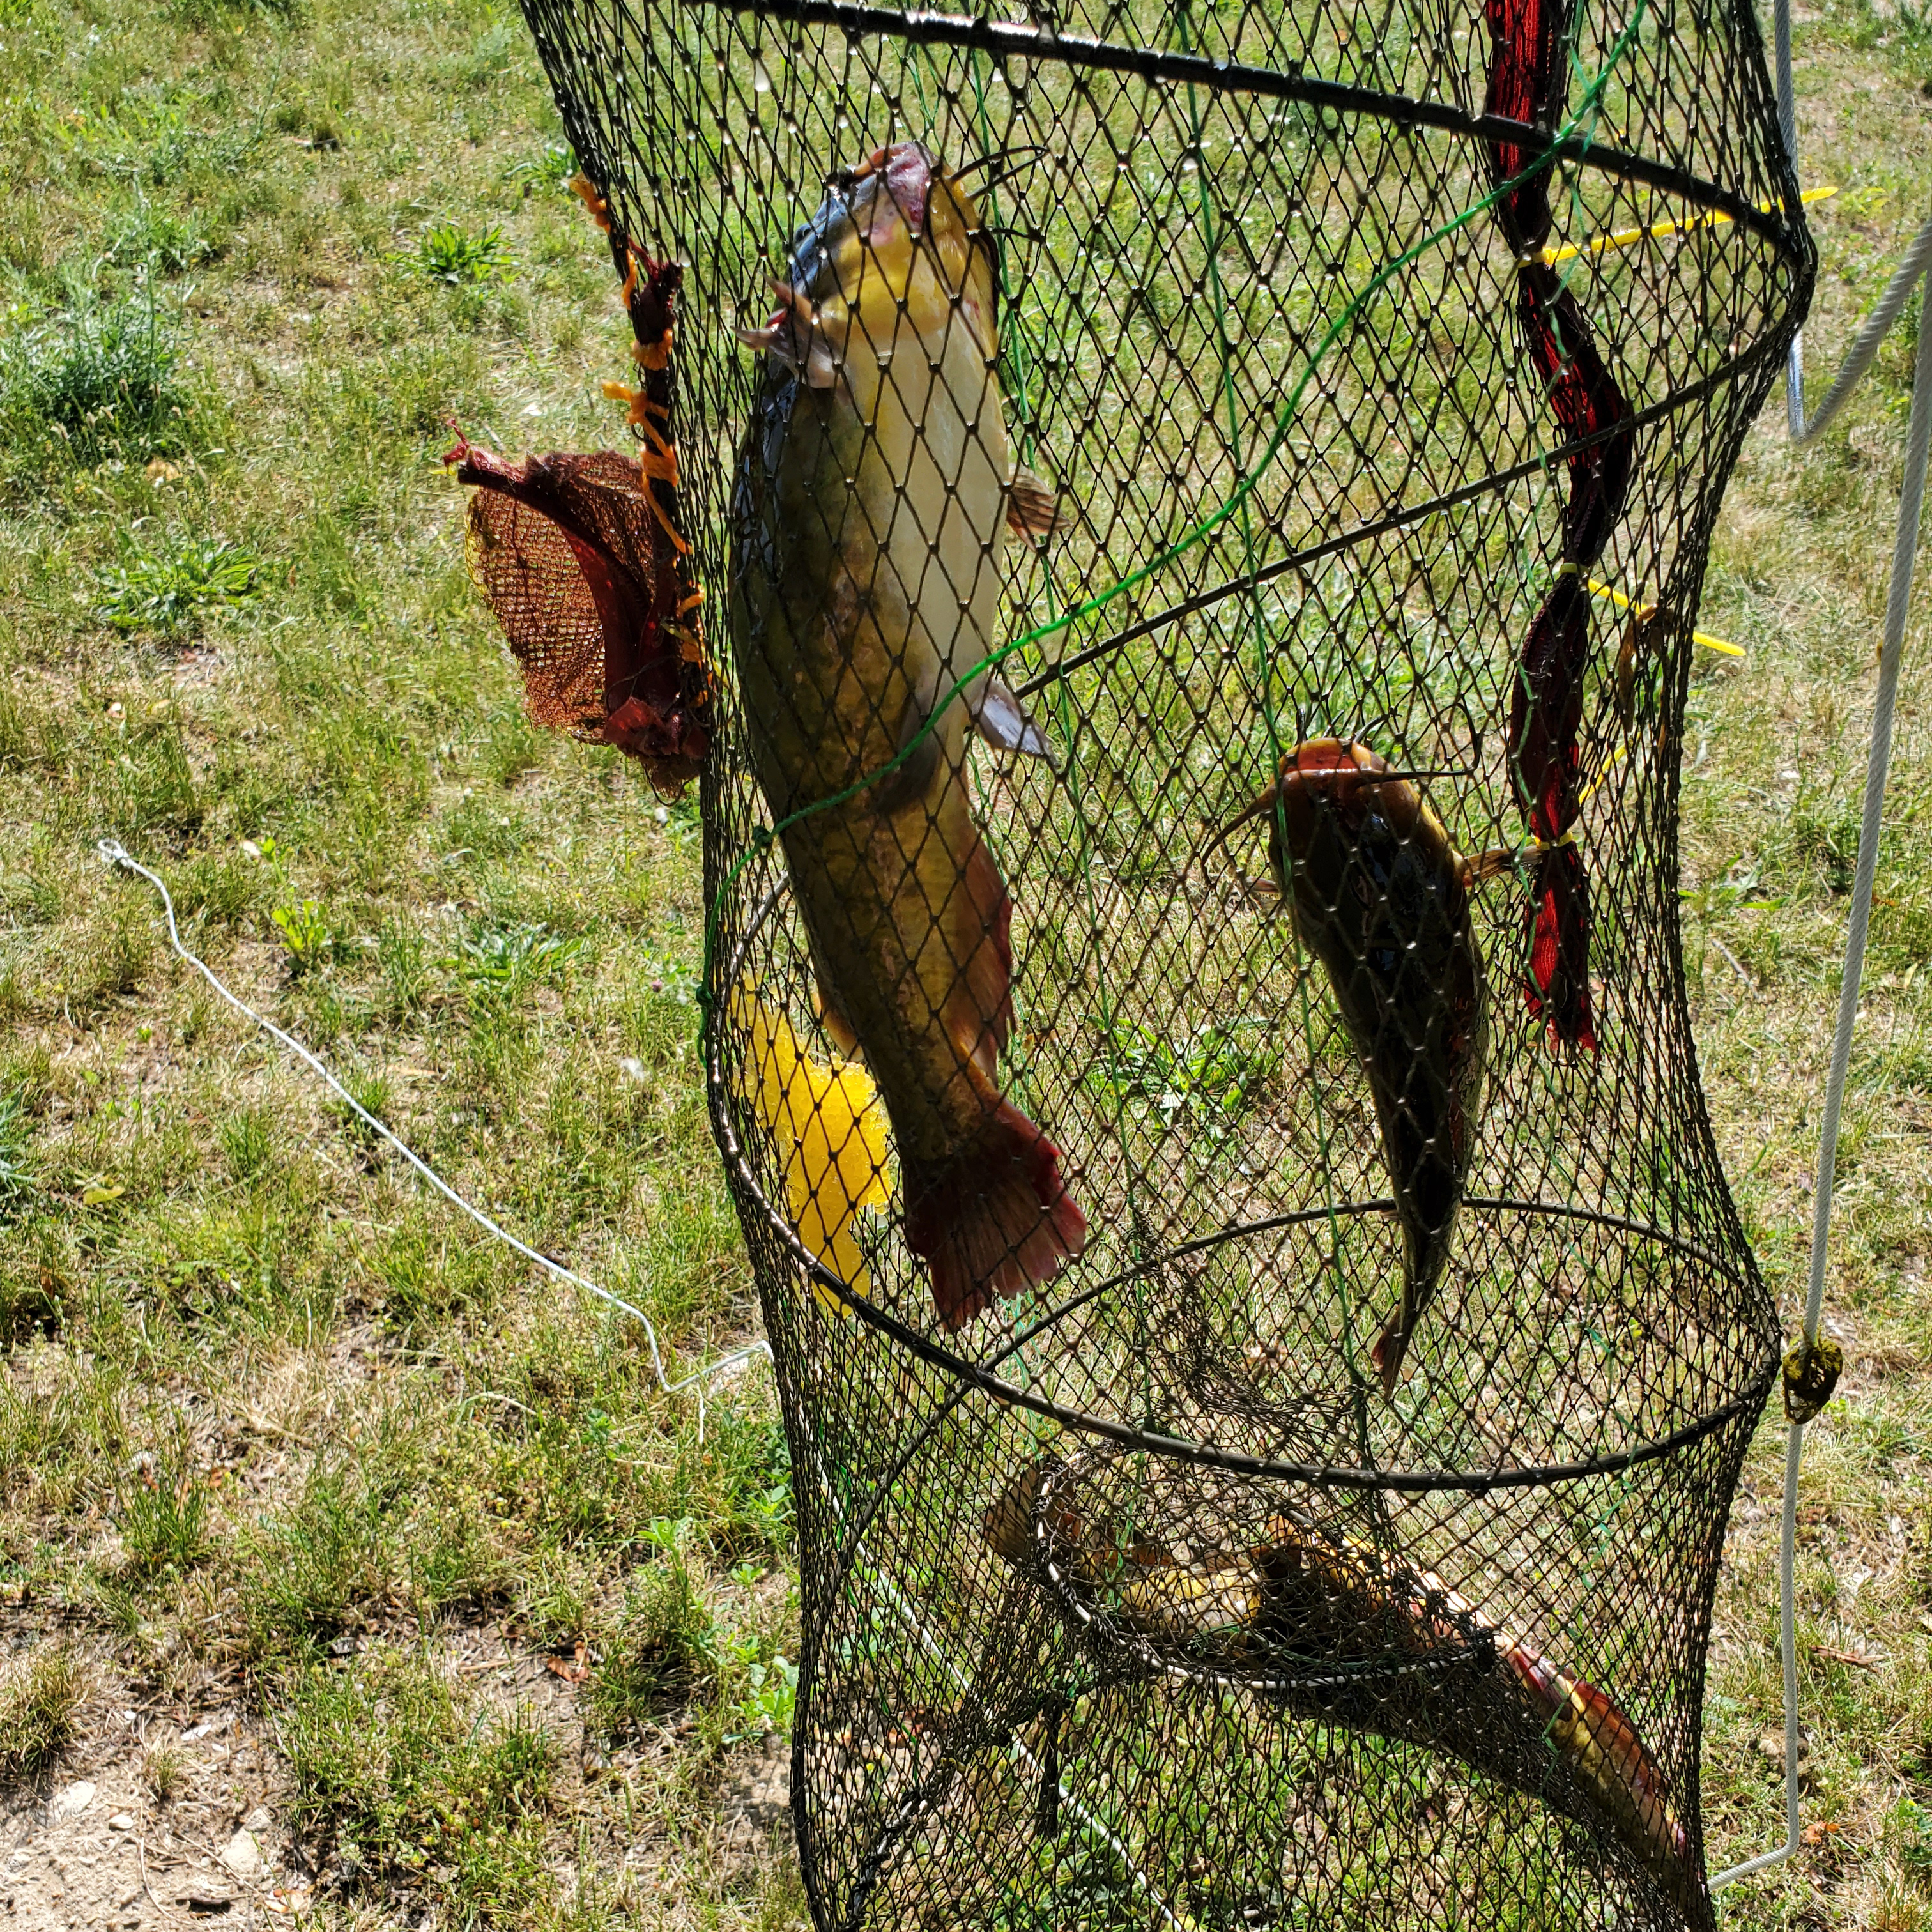
\includegraphics[width=0.7\textwidth]{F:/Funded/UIREEJ/Flint_River_Ecology/Poster/Img/Methods_00.png}
    %     \end{center}
    % \end{minipage} % \pause
    %   \begin{minipage}{0.55\textwidth}
    %     \begin{center}
    %       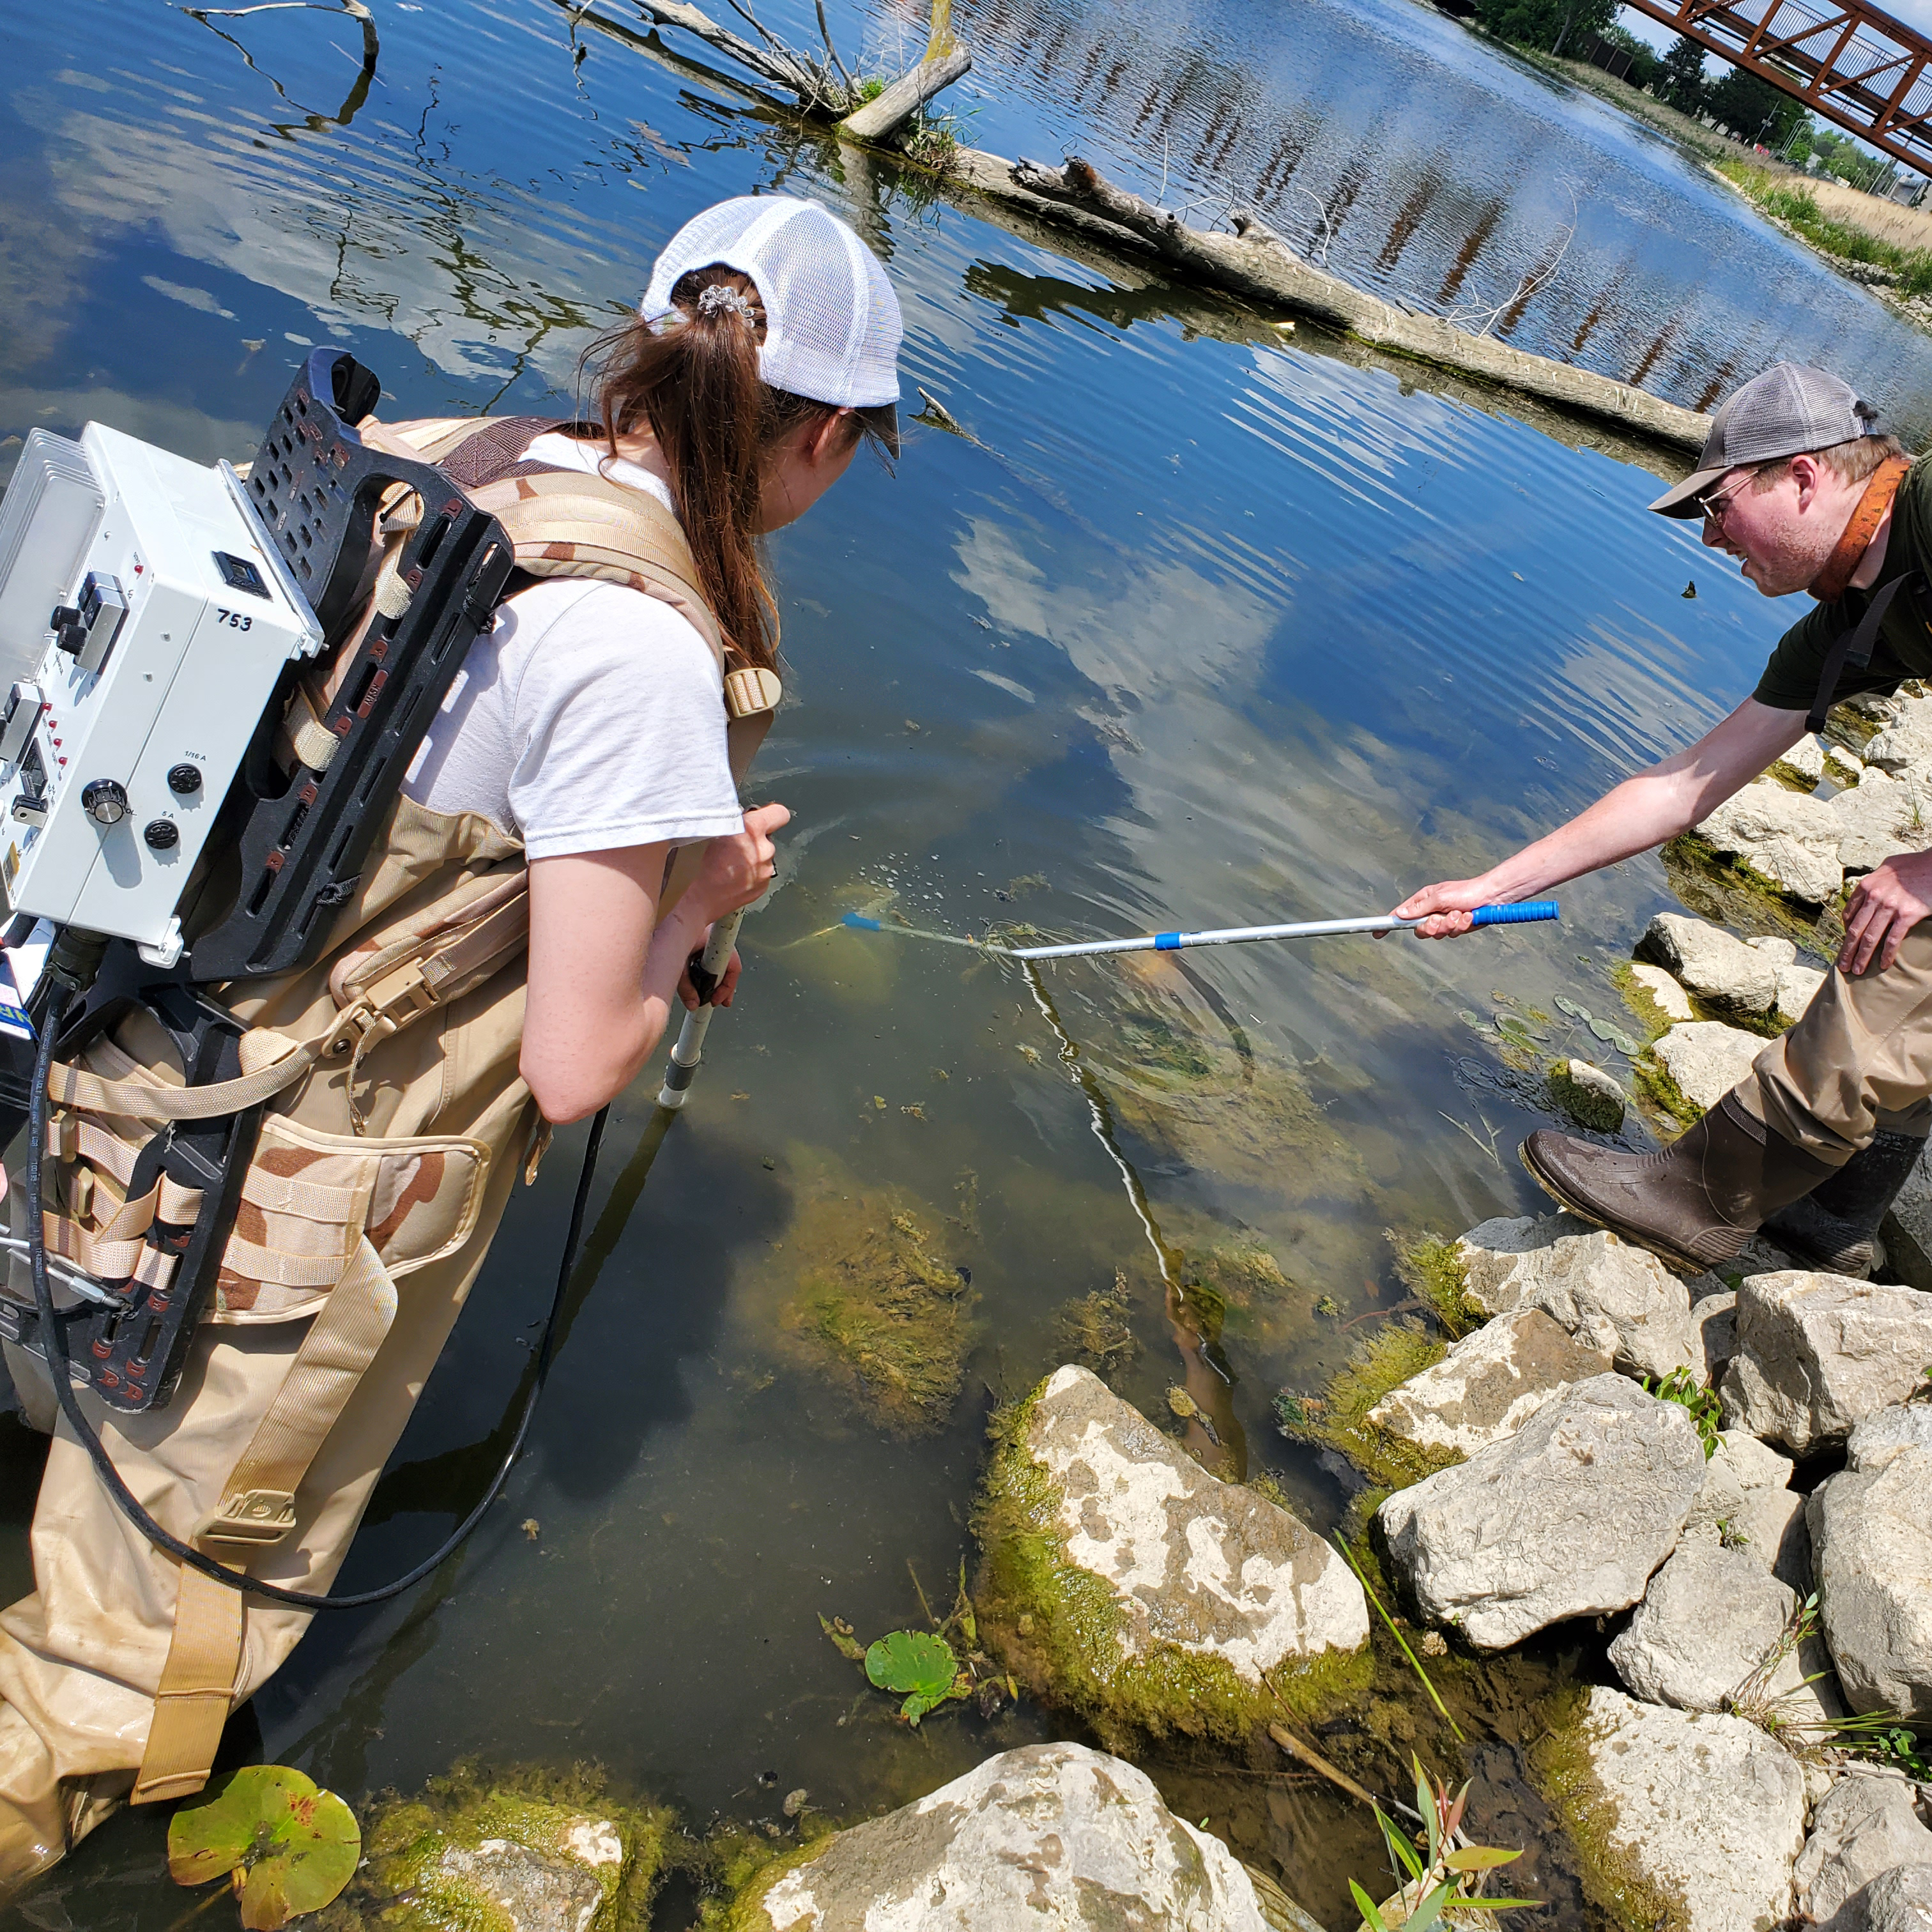
\includegraphics[width=0.93\textwidth]{F:/Funded/UIREEJ/Flint_River_Ecology/Poster/Img/Methods_01.png}
    %     \end{center}
    % \end{minipage} % \pause
    % \begin{minipage}{0.44\textwidth}
    %     \begin{center}
    %       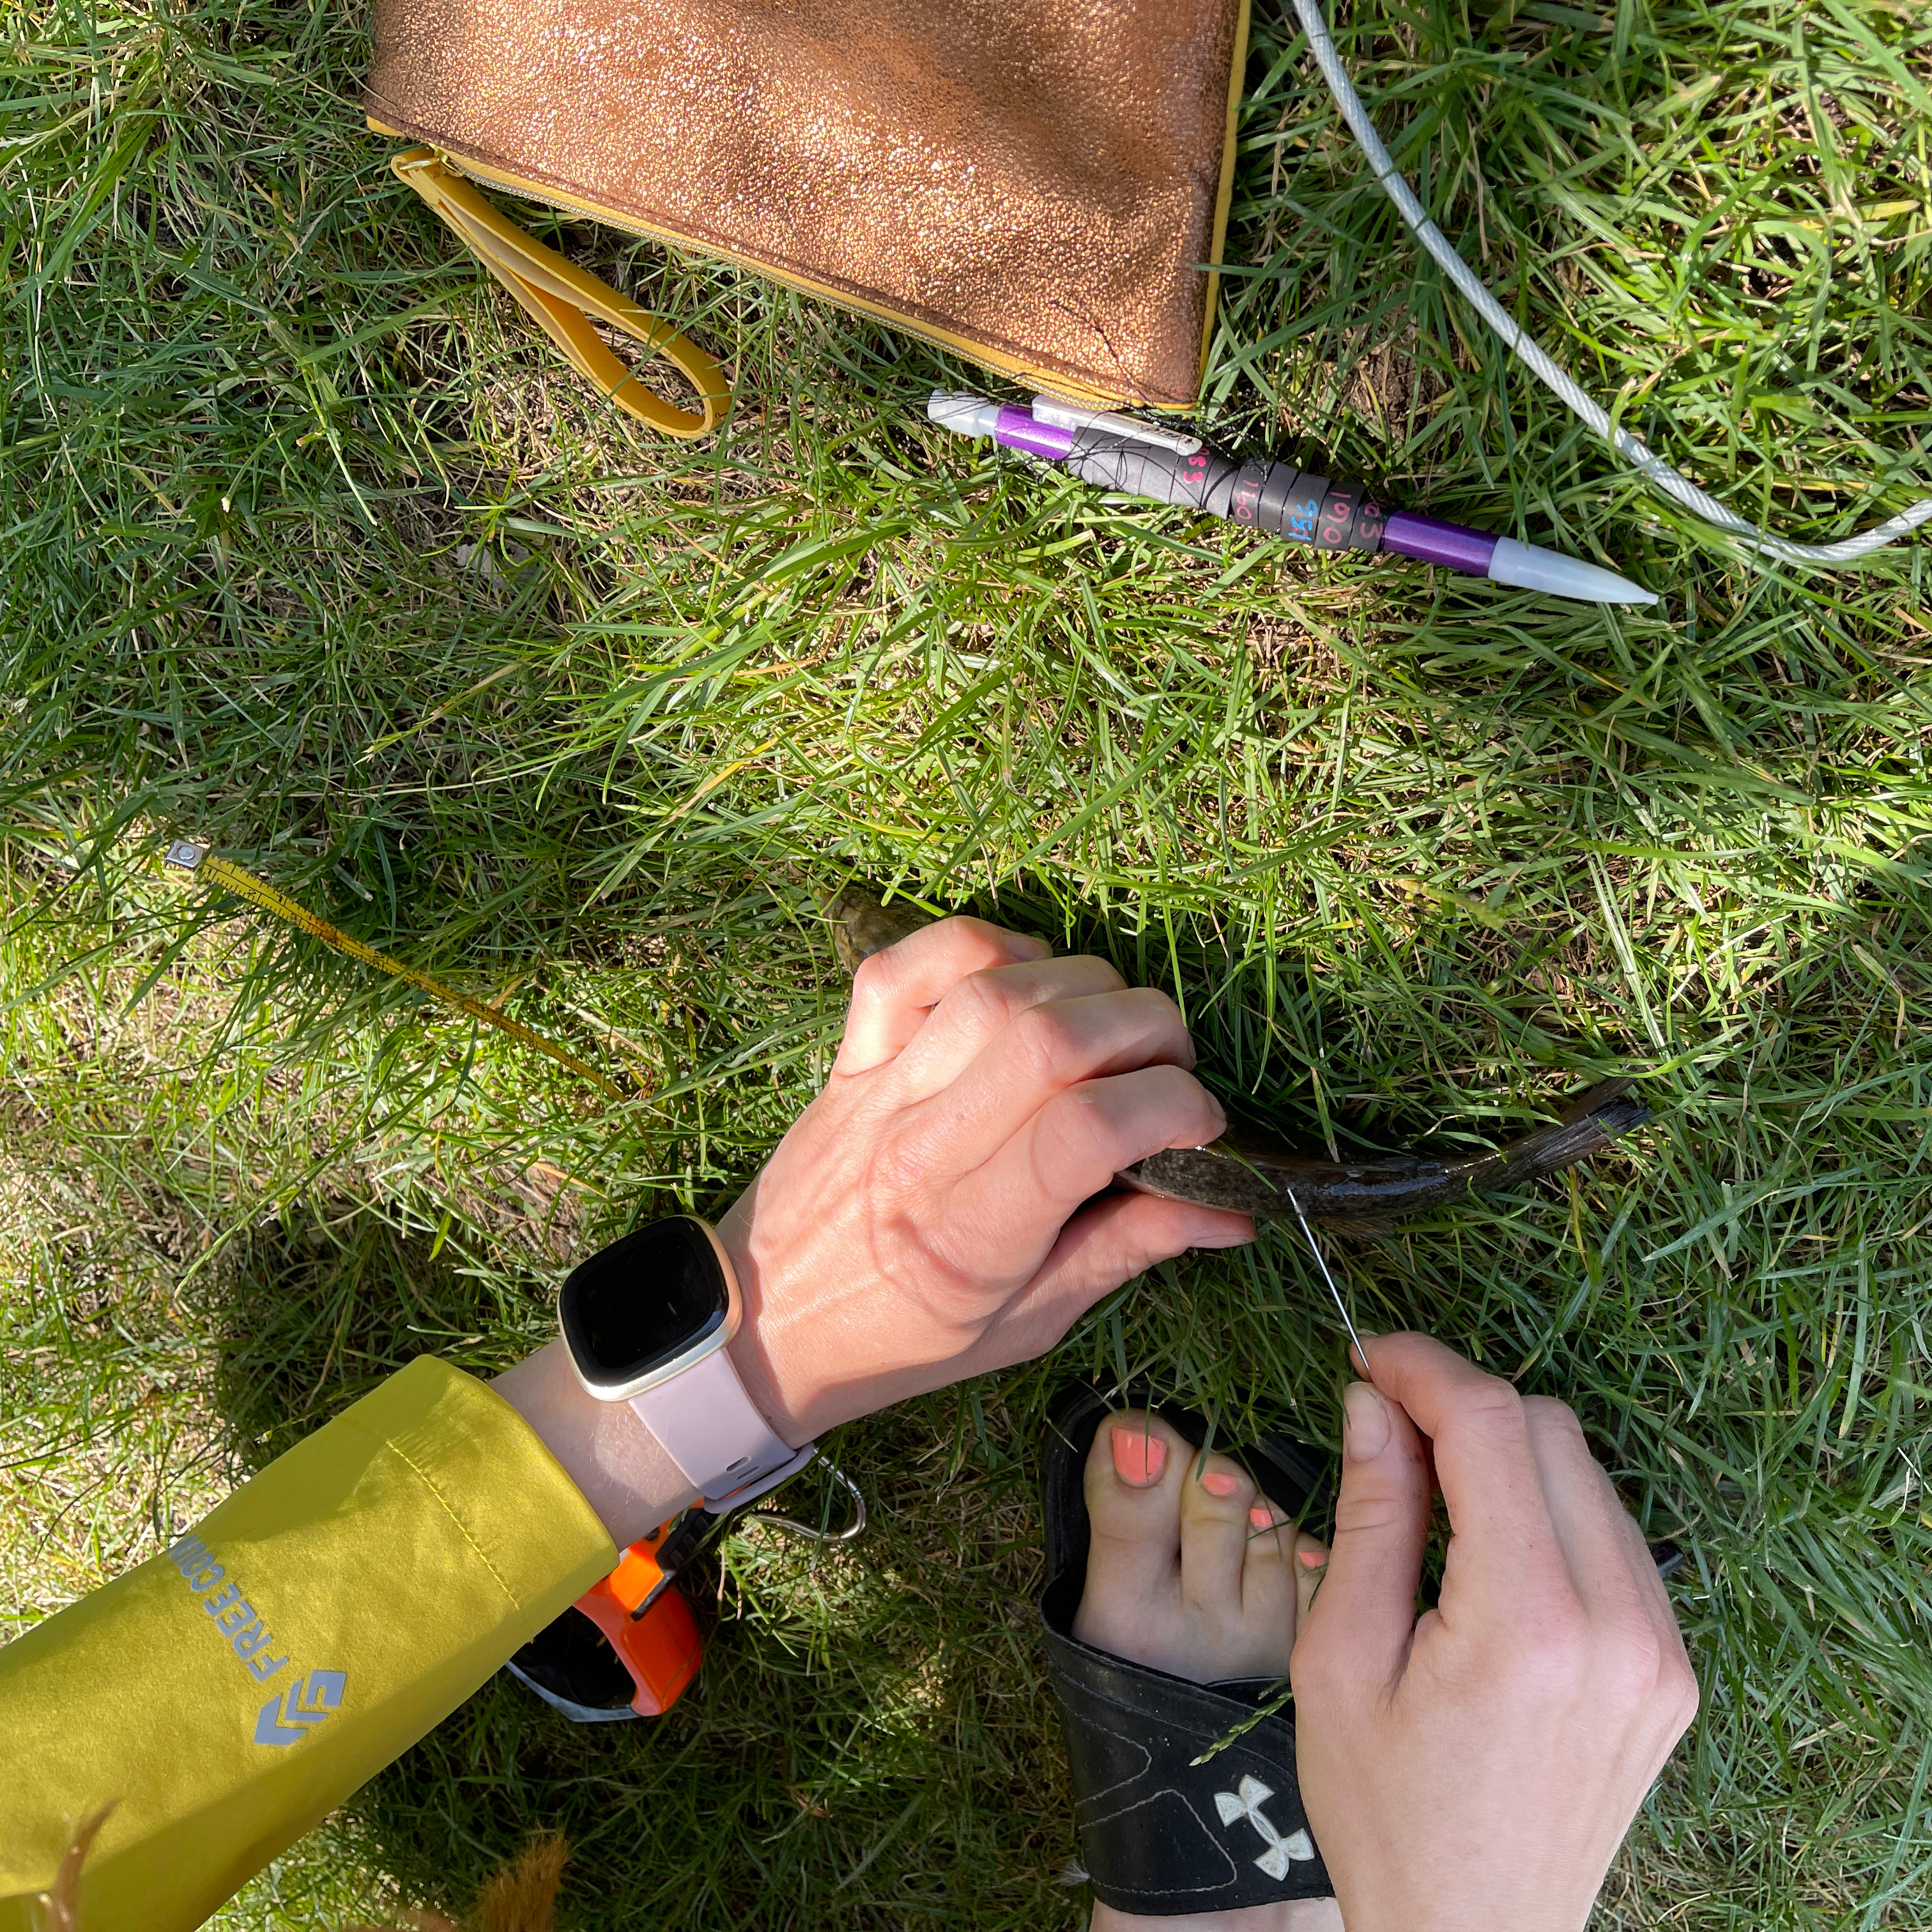
\includegraphics[width=0.7\textwidth]{F:/Funded/UIREEJ/Flint_River_Ecology/Poster/Img/Methods_10.png}
    %     \end{center}
    % \end{minipage} % \pause
    %   \begin{minipage}{0.55\textwidth}
    %     \begin{center}
    %       \includegraphics[width=0.93\textwidth]{F:/Funded/UIREEJ/Flint_River_Ecology/Poster/Img/Methods_11.png}
    %     \end{center}
    % \end{minipage} 
    % \begin{itemize}
        % \iast Flint River- (Flint, Michigan) Data was collected from four sites of the Hamilton Dam. \vspace{2.5mm} \pause
        % \iast Fish were obtained by cast nets, gillnets, hoop traps, electrofishing and hook and line. \vspace{2.5mm} \pause
        % \iast Once fish are obtained, record species, length (cm), weight (kg)  and floy tag number if length $>$ 16cm. Floy tags were added by tagging gun and a homemade floy tag method. \vspace{2.5mm} \pause
        % \iast Select fish were preserved for heavy metal analysis. \vspace{2.5mm} \pause
        % \iast The following invasives species were euthanized: Round goby, White perch, Common goldfish.
    % \end{itemize}
\end{frame}

% \begin{frame}
%     \frametitle{Methods} % \pause
    
%     \begin{minipage}{0.49\textwidth}
%         \begin{center}
%           \includegraphics[width=0.7\textwidth]{F:/Research/Funded/UIREEJ/Flint_River_Ecology/Slides/Img/-2-1.png}
%         \end{center}
%     \end{minipage} % \pause
%       \begin{minipage}{0.49\textwidth}
%         \begin{center}
%           \includegraphics[width=0.7\textwidth]{F:/Research/Funded/UIREEJ/Flint_River_Ecology/Slides/Img/-2-2.png}
%         \end{center}
%     \end{minipage} % \pause
%     \begin{minipage}{0.49\textwidth}
%         \begin{center}
%           \includegraphics[width=0.7\textwidth]{F:/Research/Funded/UIREEJ/Flint_River_Ecology/Slides/Img/-2-3.png}
%         \end{center}
%     \end{minipage} % \pause
%       \begin{minipage}{0.49\textwidth}
%         \begin{center}
%           \includegraphics[width=0.7\textwidth]{F:/Research/Funded/UIREEJ/Flint_River_Ecology/Slides/Img/-2-4.png}
%         \end{center}
%     \end{minipage} 
% \end{frame}

% \begin{frame}
%     \frametitle{Methods} % \pause
    
%     \begin{minipage}{0.49\textwidth}
%         \begin{center}
%           \includegraphics[width=0.6\textwidth]{F:/Research/Funded/UIREEJ/Flint_River_Ecology/Slides/Img/-3-1.png}
%         \end{center}
%     \end{minipage} % \pause
%       \begin{minipage}{0.49\textwidth}
%         \begin{center}
%           \includegraphics[width=0.6\textwidth]{F:/Research/Funded/UIREEJ/Flint_River_Ecology/Slides/Img/-3-3.png}
%         \end{center}
%     \end{minipage} % \pause
%     \begin{center}
%         \includegraphics[width=0.5\textwidth]{F:/Research/Funded/UIREEJ/Flint_River_Ecology/Slides/Img/-3-2.png}
%     \end{center}
% \end{frame}

% \section{Figures}

%%%%%%%%%%%%%%%%%%%%%%%%%%%%%%%%%%%%%%%%%%%%%%%%%%%%%%%%%%%%%%%%%%%%%%%%%%%%%%%%%%%%%%%%%%%%%%%%%
%%%%%  Diversity  %%%%%%%%%%%%%%%%%%%%%%%%%%%%%%%%%%%%%%%%%%%%%%%%%%%%%%%%%%%%%%%%%%%%%%%%%%%%%%%
%%%%%%%%%%%%%%%%%%%%%%%%%%%%%%%%%%%%%%%%%%%%%%%%%%%%%%%%%%%%%%%%%%%%%%%%%%%%%%%%%%%%%%%%%%%%%%%%%

% \subsection{Diversity}

\begin{frame}
    \frametitle{Diversity} % \pause
    \begin{center} 
        \includegraphics[width=1.0\textwidth]{F:/Funded/UIREEJ/Flint_River_Ecology/Poster/Img/Diversity_Bubble_Plot_T.png} \\
    \end{center}
    
    % In this figure we compare catch rates between sites $ 1 \& 3 $ below the dam, and sites $ 2 \& 4 $ above the dam. 
    % Notable differences show much higher catch rates of gizzard shad below the dam and rock bass above the dam.
\end{frame}

%%%%%%%%%%%%%%%%%%%%%%%%%%%%%%%%%%%%%%%%%%%%%%%%%%%%%%%%%%%%%%%%%%%%%%%%%%%%%%%%%%%%%%%%%%%%%%%%%
%%%%%  Toxins  %%%%%%%%%%%%%%%%%%%%%%%%%%%%%%%%%%%%%%%%%%%%%%%%%%%%%%%%%%%%%%%%%%%%%%%%%%%%%%%%%%
%%%%%%%%%%%%%%%%%%%%%%%%%%%%%%%%%%%%%%%%%%%%%%%%%%%%%%%%%%%%%%%%%%%%%%%%%%%%%%%%%%%%%%%%%%%%%%%%%

% \subsection{Toxins}

\begin{frame}
    \frametitle{Toxins} % \pause
    \begin{center}
        \includegraphics[width=0.9\textwidth]{F:/Funded/UIREEJ/Flint_River_Ecology/Poster/Img/Hg.png} \\
    \end{center}
    
    % In this figure we compare Hg levels from tested fish caught between sites $ 1 \& 3 $ below the dam, and sites $ 2 \& 4 $ above the dam. 
    % The values represent the difference between downstream and upstream species tested. e.g $ (downstream - upstream) $ mg/kg.
\end{frame}

\section{Results}

%%%%%%%%%%%%%%%%%%%%%%%%%%%%%%%%%%%%%%%%%%%%%%%%%%%%%%%%%%%%%%%%%%%%%%%%%%%%%%%%%%%%%%%%%%%%%%%%%
%%%%%  Discussion 1  %%%%%%%%%%%%%%%%%%%%%%%%%%%%%%%%%%%%%%%%%%%%%%%%%%%%%%%%%%%%%%%%%%%%%%%%%%%%
%%%%%%%%%%%%%%%%%%%%%%%%%%%%%%%%%%%%%%%%%%%%%%%%%%%%%%%%%%%%%%%%%%%%%%%%%%%%%%%%%%%%%%%%%%%%%%%%%

% \subsection{Discussion 1}

% \begin{frame}
%     \frametitle{Discussion} % \pause
%     \begin{itemize}
%         \iast Using Simpson's Diversity Index we compared species diversity above and below the dam.
%         We computed relative index values for the four sites $ (S), D_{S_{3}} = 0.48 \le D_{S_{4}} = 0.72 \le D_{S_{1}} = 0.77 = D_{S_{2}} = 0.77 $. \vspace{2.5mm} \pause
%         \iast Downstream yielded an index of 0.67 with 31 species caught. 
%         The overall catch was dominated by Gizzard shad making it less even than upstream. \vspace{2.5mm} \pause
%         \iast Upstream yielded an index of 0.75 with 20 species caught. 
%         Though there was less species diversity, it yielded a higher index because there was more eveness among the species caught.
%     \end{itemize}
% \end{frame}

%%%%%%%%%%%%%%%%%%%%%%%%%%%%%%%%%%%%%%%%%%%%%%%%%%%%%%%%%%%%%%%%%%%%%%%%%%%%%%%%%%%%%%%%%%%%%%%%%
%%%%%  Discussion 2  %%%%%%%%%%%%%%%%%%%%%%%%%%%%%%%%%%%%%%%%%%%%%%%%%%%%%%%%%%%%%%%%%%%%%%%%%%%%
%%%%%%%%%%%%%%%%%%%%%%%%%%%%%%%%%%%%%%%%%%%%%%%%%%%%%%%%%%%%%%%%%%%%%%%%%%%%%%%%%%%%%%%%%%%%%%%%%

% \subsection{Discussion 2}

% \begin{frame}
%     \frametitle{Discussion} % \pause
%     \begin{itemize}
%         \iast The dam prevents species from traveling upstream, we caught more species below the dam. 
%         Fishing methods upstream differed from downstream due to the different habitats. 
%         This could impact the fish species caught and the quantities. \vspace{2.5mm} \pause
%         \iast Mercury levels were analyzed in fish above and below the dam.
%         Bass contained higher levels of mercury compared to other species. 
%         Fish higher in the trophic level bioaccumulate more than other species. 
%         Downstream had more species with higher levels of mercury. 
%         This could be due to downstream containing species that are migrating from The Great Lakes.
%     \end{itemize}
% \end{frame}

\section{Conclusion}

%%%%%%%%%%%%%%%%%%%%%%%%%%%%%%%%%%%%%%%%%%%%%%%%%%%%%%%%%%%%%%%%%%%%%%%%%%%%%%%%%%%%%%%%%%%%%%%%%
%%%%%  Conclusion  %%%%%%%%%%%%%%%%%%%%%%%%%%%%%%%%%%%%%%%%%%%%%%%%%%%%%%%%%%%%%%%%%%%%%%%%%%%%%%
%%%%%%%%%%%%%%%%%%%%%%%%%%%%%%%%%%%%%%%%%%%%%%%%%%%%%%%%%%%%%%%%%%%%%%%%%%%%%%%%%%%%%%%%%%%%%%%%%

% \subsection{Conclusion}

\begin{frame}
    \frametitle{Conclusion} % \pause
    \textbf{ \Large \hspace{5mm}
        The ecology study of the Flint River has been conducted for 2 years. 
        Study will be continued through the removal of the Hamilton Dam and restoration of the Flint River. 
        This pre-assessment will be used to compare data once restoration is 
        complete to understand how dam removal impacts riverine ecosystems.
        }
\end{frame}

%%%%%%%%%%%%%%%%%%%%%%%%%%%%%%%%%%%%%%%%%%%%%%%%%%%%%%%%%%%%%%%%%%%%%%%%%%%%%%%%%%%%%%%%%%%%%%%%%
%%%%%  Acknowledgements  %%%%%%%%%%%%%%%%%%%%%%%%%%%%%%%%%%%%%%%%%%%%%%%%%%%%%%%%%%%%%%%%%%%%%%%%
%%%%%%%%%%%%%%%%%%%%%%%%%%%%%%%%%%%%%%%%%%%%%%%%%%%%%%%%%%%%%%%%%%%%%%%%%%%%%%%%%%%%%%%%%%%%%%%%%

% \subsection{Acknowledgements}

\begin{frame}
    \frametitle{Acknowledgements} % \pause
    \begin{center}
      \textbf{\Large For funding we thank \dots}
    \end{center}
    \begin{itemize}
      \iast The Community Foundation of Greater Flint
      \iast Saginaw Bay Watershed Initiative Network
      \iast UM-Flint Office of Research
      \iast UM-Flint CAS Opportunity Fund
      \iast UM-Flint Urban Institute for Racial, Economic, \& Enviornmental Justice
      \iast The Gary and Colleen Pace Field Biology Scholarship
      \iast Those who have worked on or helped with the project including many UM-Flint students, 
      Megan Heyza, and the Flint River Watershed Coalition
    \end{itemize}
\end{frame}

% \begin{frame}
%   \frametitle{Acknowledgements} % \pause
%   For funding we thank the Community Foundation of Greater Flint, 
%   Saginaw Bay Watershed Initiative Network, 
%   UM-Flint Office of Research, 
%   UM-Flint CAS Opportunity Fund, 
%   UM-Flint Urban Institute for Racial, Economic, \& Enviornmental Justice,
%   and the Gary and Colleen Pace Field Biology  Scholarship. 
%   We thank those who have worked on or helped with the project including many UM-Flint students, 
%   Megan Heyza, and the Flint River Watershed Coalition
% \end{frame}

%%%%%%%%%%%%%%%%%%%%%%%%%%%%%%%%%%%%%%%%%%%%%%%%%%%%%%%%%%%%%%%%%%%%%%%%%%%%%%%%%%%%%%%%%%%%%%%%%
%%%%%  References  %%%%%%%%%%%%%%%%%%%%%%%%%%%%%%%%%%%%%%%%%%%%%%%%%%%%%%%%%%%%%%%%%%%%%%%%%%%%%%
%%%%%%%%%%%%%%%%%%%%%%%%%%%%%%%%%%%%%%%%%%%%%%%%%%%%%%%%%%%%%%%%%%%%%%%%%%%%%%%%%%%%%%%%%%%%%%%%%

% \subsection{References}

\begin{frame}
  \frametitle{References} % \pause
    \textbf{[ 1 ]}: Bankston, N. (2014). Automobile Industry Growth from \\ 1916 to 1989: The Effect on Flint, Michigan Climate. \\ \vspace{2.5mm}
    \textbf{[ 2 ]}: Bernier, J., Brousseau, P., Krzystyniak, K., Tryphonas, H., \& Fournier, M. (1995). Immunotoxicity of heavy metals in relation to Great Lakes. Environmental health perspectives, 103 Suppl 9, 23-34. doi:10.1289/ehp.95103s923 \\ \vspace{2.5mm}
    \textbf{[ 3 ]}: McGoldrick, D. J., \& Murphy, E. W. (2016). Concentration and distribution of contaminants in lake trout and walleye from the Laurentian Great Lakes (2008–2012). Environmental Pollution, 217, 85-96. doi:https://doi.org/10.1016/j.envpol.2015.12.019 \\ \vspace{2.5mm}
    \textbf{[ 4 ]}: Hunter, J. D. (2007). Matplotlib: A 2D graphics environment. Computing in Science \& Engineering, vol. 9, no. 3, pp. 90-95. doi:https://doi.org/10.5281/zenodo.3633844
\end{frame}

\end{document} 